\chapter{Efficient knockoffs construction}\label{ch:sdp}

As shown in Chapter~\ref{ch:fs}, in the case of gaussian knockoffs
$\tX$ can be sampled from a normal distribution $\cN\left( \bupsilon,\, \Upsilon \right)$ whose parameters
$\bupsilon,\, \Upsilon$ are formulated in~\ref{eq:conditional_gaussian_knockoffs}.
\begin{equation}\label{eq:conditional_gaussian_knockoffs}
    \tcX \mid \cX \sim \cN\left( \bupsilon, \Upsilon \right)
    ,\qquad\text{where}\quad
    \begin{cases*}
        \bupsilon = \cX - \cX\Sigma^{-1}\diag(\bs)\\
        \Upsilon = \diag(\bs)\left( 2\mI_{p \times p} - \Sigma^{-1}\diag(\bs) \right)
    \end{cases*}
\end{equation}
More generally, the same parameters are derived by only imposing
$\big[ X, \tX \big]_{\swap\left( S \right)}$ and $\big[ X, \tX \big]$
to have equal first two moments
for any subset
$S \subseteq \left\{ 1, \dots, p \right\}$,
rather than the same distribution.
These formulas are valid for any vector $\bs \in \R^p$ such that $\Omega$
is indeed a covariance matrix (semidefinite positive).
\begin{equation*}
    \Omega = \begin{bmatrix}
        \Sigma & \Sigma - \diag \bs\\
        \Sigma - \diag \bs & \Sigma
    \end{bmatrix}
    \succeq \0_{2p \times 2p}
\end{equation*}
As shown in proposition~\ref{prop:omega_psd},
this matrix is semidefinite positive if and only if $\0_{p \times p} \preceq \diag \bs \preceq 2 \Sigma$.
The first inequality clearly holds if all the entries of $\bs$ are positive.
It is however trickier to identify all vectors $\bs$ satisfying the second one.

In this chapter, we show why the choice of $\bs$ is important and how to efficiently find a good one
in the high dimensional setting.
In the remaining, we note $\Sigma$ the true covariance and $\hat{\Sigma}$ its estimation from the samples $X$.

\section{Equi-correlated knockoffs}\label{sec:equi}

\subsubsection{A cheap solution}

For any psd matrix $A \in \R^p$, $A + \alpha I_{p \times p}$ has the same eigenvalues as $A$, but shifted by $\alpha$.
It gives a fast and simple way to find a feasible $\bs$.
\begin{equation}\label{eq:equi}
    s_j = \min(2\lambda_{\min}(\cove),\, 1)
    \quad\text{ for all } 0 \leq j \leq p
\end{equation}
The problem of finding the smallest eigenvalue $\lambda_{\min}(\cove)$ can be solved efficiently,
using for instance a singular value decomposition which runs in $\cO(p)$ steps~\cite{svd}.

\subsubsection{Why it is not desirable}

For large values of $p$,
the minimum eigenvalue of $\cove$ is likely to be very small,
unless $\cove$ has a substantially special structure.
Let us analyze briefly the covariance of $\big[ \cX; \tcX \big]$
to understand why it is unprofitable for the selection procedure.
If $\tcX$ is built according to~\ref{eq:conditional_gaussian_knockoffs}, it satisfies
\begin{equation*}
    \begin{cases}
        \cov(\tcX_j,\, \tcX_{j'}) = \cov(\cX_j,\, \cX_{j'}) \text{ for all } j,\,j'\\
        \cov(\cX_j,\, \tcX_{j'}) = \cov(\cX_j,\, \cX_{j'}) \text{ for all } j \neq j'\\
        \cov(\cX_j,\, \tcX_j) = \cov(\cX_j,\, \cX_j) - s_j \text{ for all } j
    \end{cases}
\end{equation*}
First, $\tcX$ has the same internal covariance has $\cX$,
and two distinct original and knockoff features have the same covariance
as the one of the two corresponding original features.
It makes the knockoff feature sufficiently close to the original features
to fool the estimator computing the statistics.
However, an original feature $j$ and its corresponding knockoff have a covariance that is smaller the larger $s_j$ is.
If $s_j$ is $0$, $\cX_j$ couldn't be distinguished from $\tcX_j$ and the selection would suffer from a low power.
It motivates us to maximize the sum of the entries of $\bs$ and it leads to solving a SDP\@.

\section{SDP knockoffs}\label{sec:sdp}

This observation motivates us to maximize the entries of $\bs$,
while maintaining the inequality $\diag\bs \preceq \tcovm$.
This can be formulated in the optimization problem~\ref{eq:sdp}.
\begin{equation}\label{eq:sdp}
    \underset{\bs \in \R^p}{\argmax}\;\,
    \sum_{j = 1}^p s_j
    \qquad
    \text{subject to } \begin{cases}
        s_j \geq 0\text{ for all } j\\
        \diag \bs \preceq \tcovm
    \end{cases}
\end{equation}
This problem is a structured semidefinite program (SDP) and can efficiently be solved for small values of
$p$ by interior point methods~\cite{interior_point_method_sdp} for example.
For larger values of $p$, even first order methods like
SCS~\cite{sdp_scs} or alternating direction~\cite{sdp_admm}
quickly become intractable.
Even though the convergence speed depends a lot on $\covm$,
it experimentally appears that alternative methods have to be considered when $p > 1000$.
The Figure~\ref{fig:cvx_sdp_times} shows the convergence time of the solvers SCS and MOSEK as a function of $p$.
Theoretically, it takes $\cO(p^3)$.

\begin{figure}
    \centering
    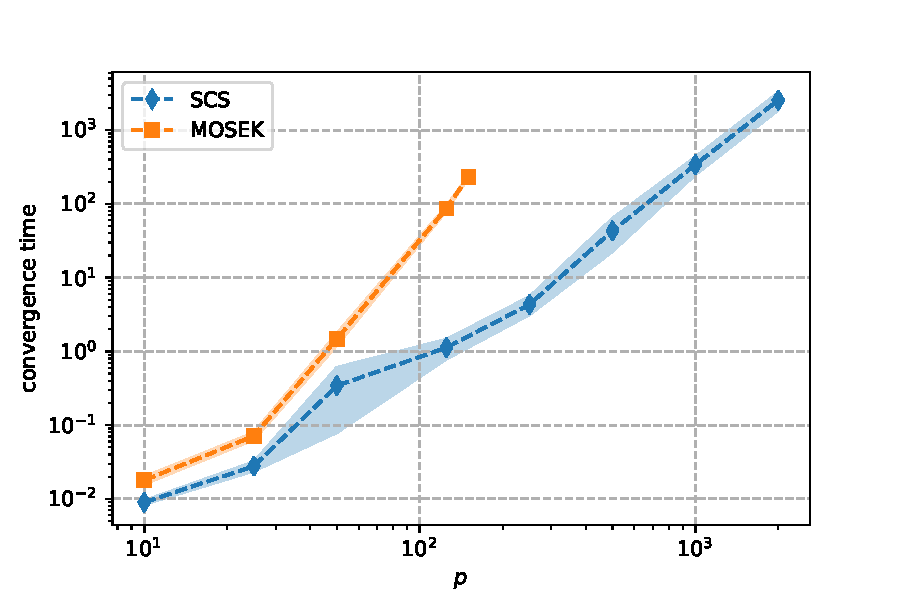
\includegraphics[width=0.8\linewidth, height=0.5\linewidth]{figures/cvx_sdp_times.pdf}
    \caption{
        Time (in seconds) required to converge for SCS (blue) and MOSEK (orange) solvers
        as a function of $p$ (in log-log scale).
        Rapidly, MOSEK needs too much memory and can't be run for $p > 150$.
        Both match the theoretical $\cO(p^3)$ rate and SCS already needs 15 minutes for $p = 1000$.
    }
    \label{fig:cvx_sdp_times}
\end{figure}

In order to reduce the computation time,
Barber-Candès suggest to solve an approximated problem of~\ref{eq:sdp} in 2 steps that we describe below.
\paragraph*{Step 1.}
Pick an approximation $\Sigma_\text{approx}$ of $\Sigma$ and solve
\begin{equation}\label{eq:sdp_approx}
    \underset{\hat{\bs} \in \R^p}{\argmax}\;\,
    \sum_{j = 1}^p \hat{s}_j
    \qquad
    \text{subject to } \begin{cases}
        \hat{s}_j \geq 0\text{ for all } j\\
        \diag \hat{\bs} \preceq \tcovmapprox
    \end{cases}
\end{equation}
\paragraph*{Step 2.}
Solve the one dimensional maximization
\begin{equation}\label{eq:sdp_approx_1d}
    \underset{\gamma \in \R}{\argmax}\;\,\gamma
    \quad\text{subject to}\quad
    \diag\left( \gamma \cdot \hat{\bs} \right) \preceq 2\Sigma
\end{equation}
Finally, pick $\bs = \gamma \cdot \hat{\bs}$.

\begin{remark}
    Note that the two extreme options $\covmapprox = \mI$ and $\covmapprox = \Sigma$ yield
    the same solutions as solving equi-knockoffs~\ref{eq:equi} and full SDP knockoffs~\ref{eq:sdp} respectively.
\end{remark}

Solving~\ref{eq:sdp_approx_1d} in step 2 can be done very efficiently using bisection as it is a one-dimensional SDP\@.
The optimization problem~\ref{eq:sdp_approx} is however the same as the one in~\ref{eq:sdp},
except for the approximation $\covmapprox$.
To speed up the computations,
$\covmapprox$ can be chosen to be a block-diagonal matrix of $k$ blocks.
The maximization then reduces to $k$ smaller SDPs for which the solutions can be found more efficiently.
These could even be distributed in several computation nodes.
Picking $\covmapprox$ is a compromise between available computation time and eventual power of the procedure.
There is a priori no ideal way to to it.
The block diagonal assumption depends on the order of the features.
They should therefore be reordered ahead of time,
typically by performing a clustering step to group very similar features.

\section{Low-rank covariance matrix approximation}\label{sec:low_rank_sigma}

A~\cite{big_data_low_rank}

\subsection{Efficient SDP solving}\label{subsec:low_rank_sdp}

\begin{algorithm}
    \caption{Forecast shifting}\label{alg:forecast_shifting}
    \begin{algorithmic}[1]
        \State \textbf{Input:} Approximation $\cove = D + U \Lambda U^\top$
        \item[]
        \State $z'_t \gets \text{quantile}_\alpha(z_t) \; \forall t$ \algorithmiccomment{\emph{(i)}}
        \For{$t = n - 1,\dots, 1$}
        \State $z'_t := \max(z'_t, z'_{t + 1} - \hat{\rho})$
        \EndFor
        \item[]
        \State $\Delta_t \gets z'_t - z'_{t - 1}\; \forall t$ for $t = 2,\dots, n$ and $\Delta_1 = z'_1 - r_0$
        \algorithmiccomment{\emph{(ii)}}
        \State $\mathbf{r^+},\,\mathbf{r^-} \gets \max(\mathbf{\Delta}, 0),\,\min(\mathbf{\Delta}, 0)$
        \item[]
        \State Shift $\mathbf{r^+}$ and $\mathbf{r^-}$ in the past according to $\mathbb{E}$
        and $\mathbb{E}$ respectively and request them.
    \end{algorithmic}
\end{algorithm}

\subsection{Efficient low-rank sampling}\label{subsec:low_rank_sampling}

The estimated covariance $\cove$ is $p \times p$ and the problem becomes intractable when $p$ is large.
The covariance matrix $\Sigma$ is approximated by a diagonal $D \in \R^{p \times p}$ plus a low rank.
\begin{equation*}
    \Sigma = D + UU^\top,
    \qquad
    \text{where }
    U \in \R^{p \times k}
\end{equation*}
The joint vector $\big[ \cX,\, \tcX \big]$ is supposed to follow a normal
$\cN\left( \0_{2p \times 2p},\, \Omega \right)$
where
\begin{equation*}
    \Omega = \begin{bmatrix}
                 \Sigma & \Sigma - \diag \bs\\
                 \Sigma - \diag \bs & \Sigma
    \end{bmatrix}
\end{equation*}
and $\bs$ is the vector returned by the SDP\@.
Note $S = \diag\bs$.
As we sample from $\cX \mid \tcX$,
we need to sample from a normal with the following parameters
\begin{equation*}
    \tcX \mid \cX \sim \cN\left( \bupsilon, \Upsilon \right)
    ,\qquad\text{where}\quad
    \begin{cases*}
        \bupsilon = \cX - \cX\Sigma^{-1}S\\
        \Upsilon = 2S - S\Sigma^{-1}S
    \end{cases*}
\end{equation*}
Using the Sherman-Morrison-Woodbury formula we get
\begin{align*}
    \Sigma^{-1} &= (D + UU^\top)^{-1}\\
    &= D^{-1} - D^{-1}U(I_k + U^\top D^{-1}U)^{-1}U^\top D^{-1}
\end{align*}
Note $(I_k + U^\top D^{-1}U)^{-1} = LL^\top$, $V = SD^{-1}UL$ and $C = 2S - SD^{-1}S$
($L$ can be computed efficiently if $k$ is small).
Then
\begin{equation*}
    \Upsilon = C + VV^\top
\end{equation*}
$C$ is diagonal and $VV^\top$ rank $k$.
Using Cholesky updates has two issues here:
\textit{(i)} $C$ is not necessarily psd which makes Cholesky rank-1 updates unstable or even infeasible,
and \textit{(ii)} the updates of the Cholesky factor are not low rank,
which means we have to store the full matrix and it's not desirable if $p$ is large.
But if $\cX \sim \cN\left( \0,\, I \right)$,
$A\cX \sim \cN\left( \0,\, AA^\top \right)$ even if $A$ is not triangular.
So we don't need a Cholesky decomposition but just a factorization of the form $MM^\top$.

The fact that $C$ is not necessarily psd is painful and I found no other solution
than sampling from a complex gaussian.
Let $H$ be a square-root of $C$ (with potentially imaginary numbers on the diagonal),
and $P = H^{-1}V$.
Then,
\begin{equation*}
    \Upsilon = H(I_{p \times p} + PP^\top)H^\top
\end{equation*}
Here using Cholesky rank-1 updates on $I_{p \times p} + PP^\top$ would be possible but
we would have to store a $p \times p$ matrix which is not good if $p$ is large.
Another factorization is possible;
note
\begin{equation*}
    W = \left(I_{k \times k} + \sqrt{I_{k \times k} + P^\top P}\right)^{-1}
\end{equation*}
Then
\begin{equation*}
    I_{p \times p} + PP^\top = BB^\top
    ,\qquad
    \text{where}
    \quad
    B = I_{p \times p} + PWP^\top
\end{equation*}
$B$ is $p \times p$ but we never have to fully evaluate it (only multiply by its internal factors).

Finally, we note $M = HB$ and we have $\Upsilon = MM^\top$.
$M$ is complex but if $\cX \sim \cN(\0,\, I)$ and $\cY = i\cX$,
then $\operatorname{Im}\left( M\cY \right) \sim \cN(\0,\, MM^\top = \Upsilon)$.
It's not very optimal because multiplications with complex numbers are more costly.
It looks like it's possible to avoid using them though, but the performance gain would be marginal.
Using this scheme, with $p = 15\,000$ and $k = 100$ we can draw $n = 5\,000$ samples in $\approx 4.1$ seconds,
while the naive method not taking into account the low rank approximation would need $\approx 185$ seconds.
(In comparison sampling $5000 \times 15\,000$ numbers from $\cN(0, 1)$ takes $\approx 2.1$ seconds)
It scales pretty well for larger $p$, $k$ and $n$ but I can't compare to the naive method as it takes too much
memory.


\begin{figure}
    \centering
    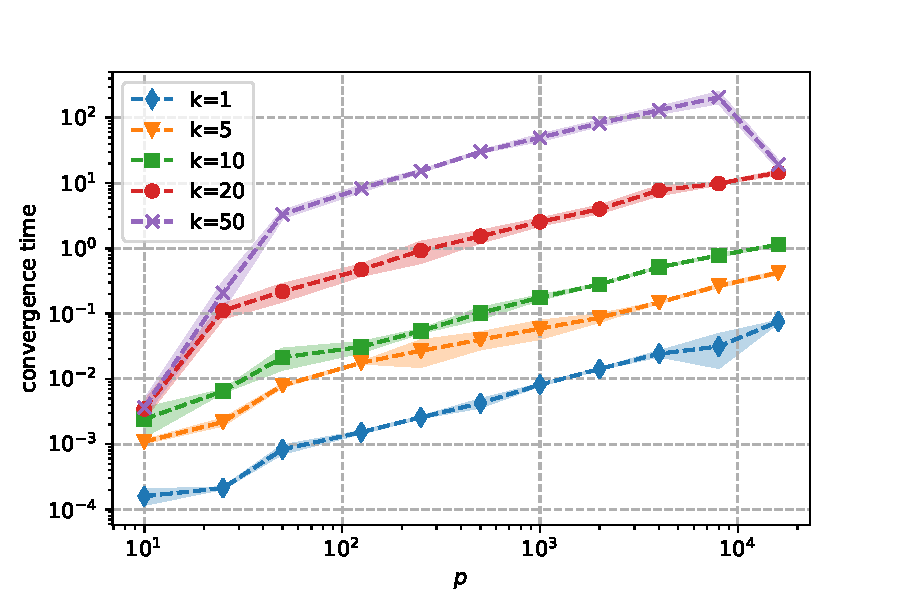
\includegraphics[width=0.8\linewidth, height=0.5\linewidth]{figures/low_rank_times.pdf}
    \caption{
    }
    \label{fig:low_rank_times}
\end{figure}